\section{(8 points)}\label{ex:apa}

L'Allocation Personnalisée à l'Autonomie en établissement (APA en établissement) est une allocation destinée aux personnes âgées de plus de 60 ans en perte d'autonomie et résidant dans un établissement de santé.


Dans cet exercice, on modélise de deux façons différentes l'évolution du montant de l'APA en établissement dans un département français.

\subsection{}

Le tableau suivant donne les montants en euro de l'APA en établissement de 2007 à 2015 pour le département considéré :

\begin{table}[h!]
	{\small \begin{tabular}{|@{\ }c@{\ }|@{\ }c@{\ }|@{\ }c@{\ }|@{\ }c@{\ }|@{\ }c@{\ }|@{\ }c@{\ }|@{\ }c@{\ }|@{\ }c@{\ }|@{\ }c@{\ }|@{\ }c@{\ }|}
	\hline
	Année                   & 2007        & 2008        & 2009        & 2010        & 2011        & 2012        & 2013        & 2014        & 2015        \\ \hline
	Rang de l'année ($x_i$) & 1           & 2           & 3           & 4           & 5           & 6           & 7           & 8           & 9           \\ \hline
	Montant, en euro de     &             &             &             &             &             &             &             &             &             \\ 
	l'APA en établissement  & \num{13504} & \num{14443} & \num{14914} & \num{15351} & \num{15751} & \num{16144} & \num{16744} & \num{17190} & \num{18070} \\ 
	($y_i$)                 &             &             &             &             &             &             &             &             &             \\ \hline
\end{tabular}}

\end{table}
En annexe \ref{sec:nuage}, à rendre avec la copie, on a représenté, dans un repère orthogonal, le nuage de points de coordonnées $(x_i ; y_i)$ associé à cette série statistique.

\begin{questions}
	
	\question
	\begin{parts}
		\part Déterminer les coordonnées du point moyen $G$ de ce nuage de points. Arrondir l'ordonnée à l'unité.
		\begin{solution}
			
			\begin{equation*}
			\bar{x} = \dfrac{1 + 2 + 3 + 4 + 5 + 6 + 7 + 8 + 9}{9} = 5
			\end{equation*}
			
			
			\begin{footnotesize}
				\begin{equation*}
				\bar{y} = \dfrac{\num{13504} + \num{14443} + \num{14914} + \num{15351} + \num{15751} + \num{16144} + \num{16744} + \num{17190} + \num{18070}}{9} \approx \num{15790.1}
			\end{equation*}
			\end{footnotesize}
			
			Le point moyen du nuage est $G(5 ; \num{15790})$.
		\end{solution}
	
		\part Placer le point $G$ dans le repère précédent.
	\end{parts}

	\question On admet que la droite $D$ d'équation $y=\num{516}x + \num{13210} $ réalise un bon ajustement affine du nuage de points jusqu'en 2020.
	
		\begin{parts}
			\part Tracer la droite $D$ dans le repère précédent. Donner les coordonnées des points choisis pour la tracer.
			
			\begin{solution}
				Soit A, le point de la droite $D$, d'abscisse 0, on a $A(0 ; y_A) $.
				
				\begin{eqnarray*}
					y_A &=& 516 \times x_A + \num{13210} \\
					y_A &=& 516 \times 0 + \num{13210} \\
					y_A &=& \num{13210} \\
				\end{eqnarray*}
			
				Pour tracer la droite $D$, j'utilise donc les points $A(0;\num{13210})$ et $G(5 ; \num{15790})$.
				
				\begin{center}
					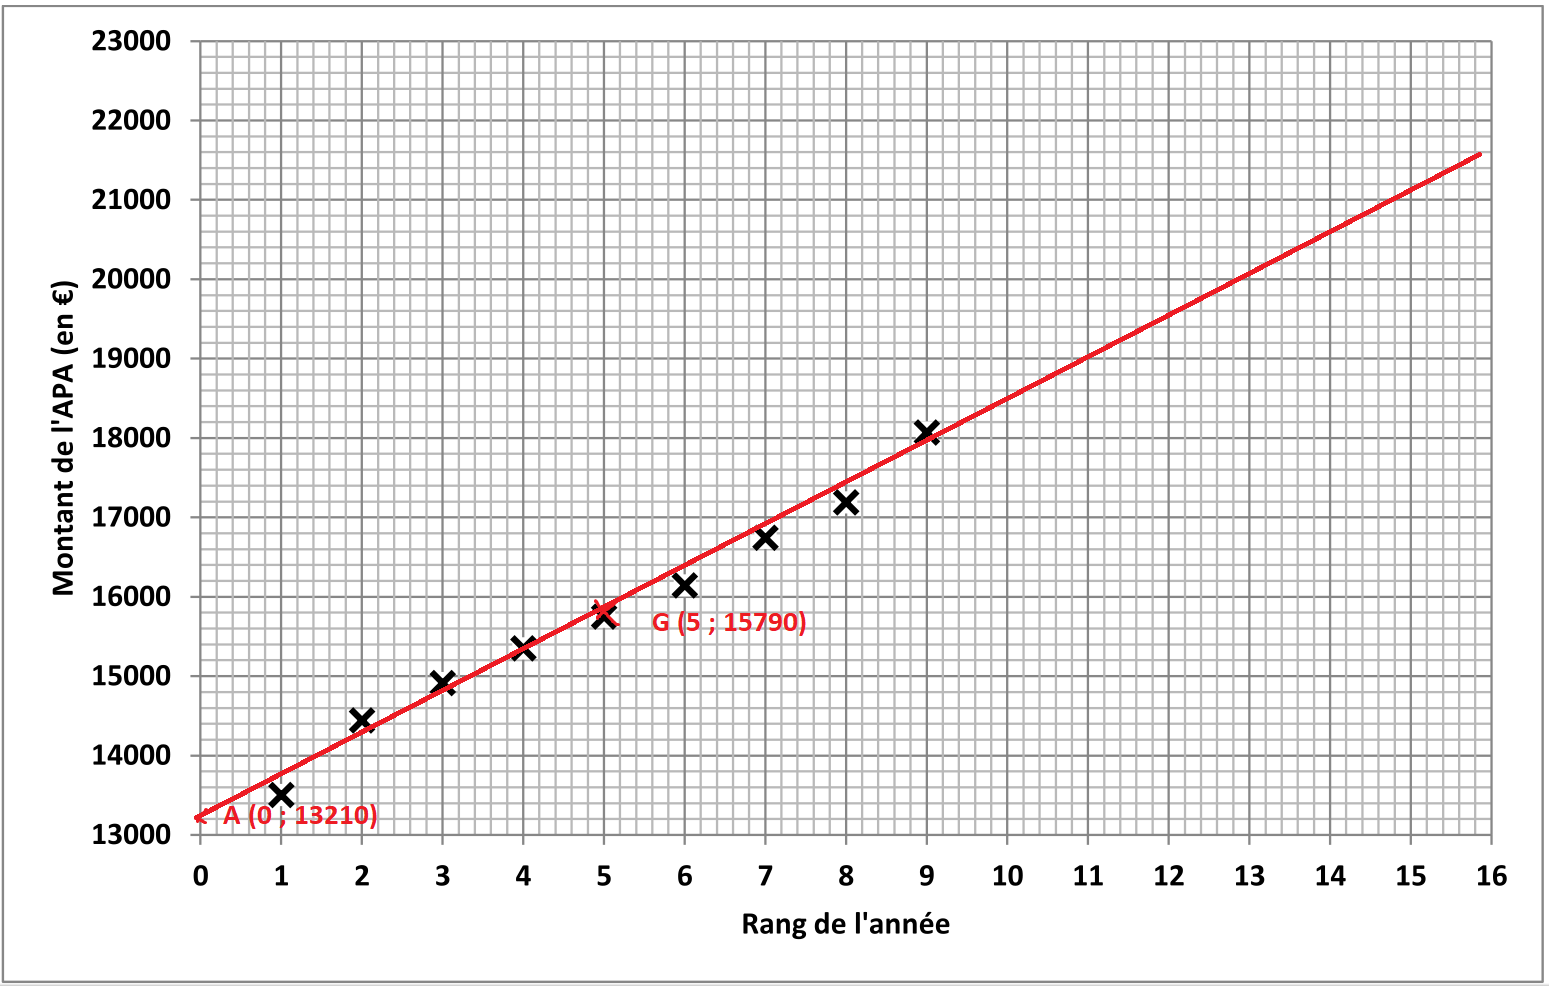
\includegraphics[scale=0.35]{img/graph_corr}
				\end{center}
			\end{solution}
			
			\part \`A l'aide de cet ajustement, donner une estimation du montant de l'APA en établissement dans ce département pour l'année 2018.
			
			\begin{solution}
				2018 est l'année de rang 12. Dans l'équation de la droite, je remplace donc $x$ par 12.
				
				\begin{eqnarray*}
					y &=& 516 \times 12 + \num{13210} \\
					y &=& \num{19402} \\
				\end{eqnarray*}
			
				On peut donc estimer que le montant de l'APA en établissement dans ce département en 2018 sera de \num{19402} €.
			\end{solution}
		\end{parts}
\end{questions}

%\newpage
\subsection{}

On a recopié le tableau précédent dans une feuille de calcul d'un tableur.
Les cellules de la ligne 4 sont au format pourcentage.

\begin{center}
	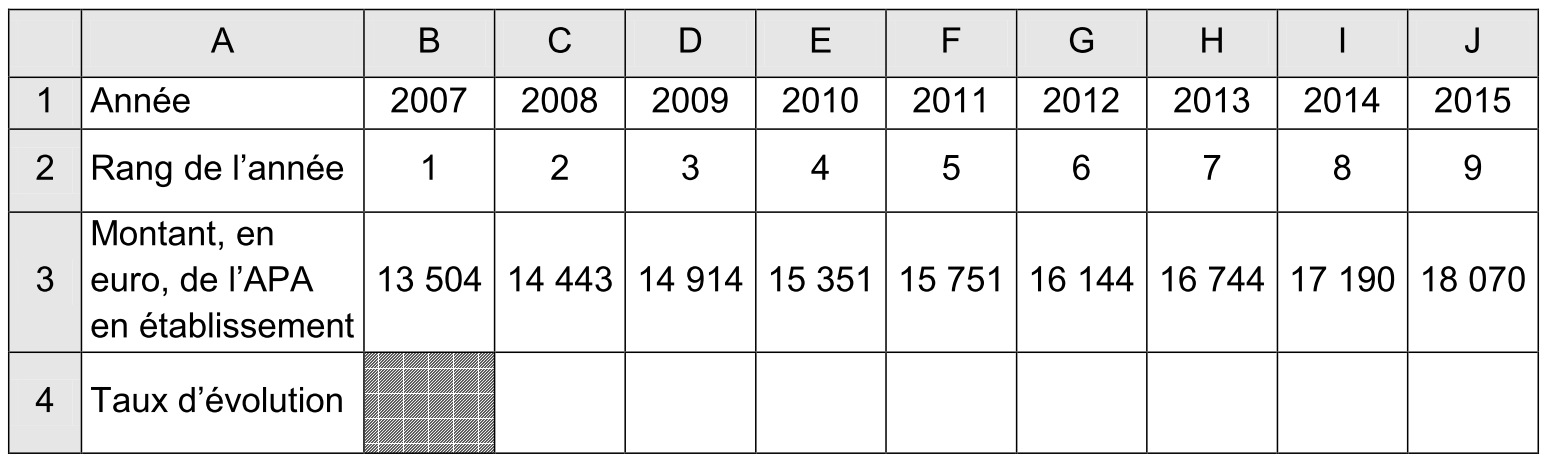
\includegraphics[scale=0.4]{img/tab_apa}
\end{center}


\begin{questions}
	\question 
		\begin{parts}
			\part Calculer le taux d'évolution de montant de l'APA en établissement dans ce département entre 2014 et 2015. Arrondir le résultat à \num{0.1} \%.
			\begin{solution}
				\begin{eqnarray*}
					t &=& \dfrac{v_{arrivée} - v_{départ}}{v_{départ}} \\
					t &=& \dfrac{\num{18070} - \num{17190}}{\num{17190}} \\
					t &\approx&  \num{0.051}
				\end{eqnarray*}
				
				Entre 2014 et 2015; l'APA en établissement a augmenté de \num{5.1} \% dans ce département.
			\end{solution}
			
			\part Quelle formule doit-on entrer dans la case $C4$ pour obtenir, par recopié vers la droite, les taux d'évolution en pourcentage du montant de l'APA en établissement dans ce département, entre deux années consécutives ?
			
			\begin{solution}
				Pour calculer le taux d'évolution on rentre en $C4$ la formule suivante : \\ $=(C3 - B3)/B3$.				
			\end{solution}
		\end{parts}
	
	
	\question On suppose maintenant que le montant de l'APA en établissement dans ce département augmente de \num{5.1} \% par an après 2015. On décide de modéliser ce montant par une suite numérique $(u_n)$.
	
	
		
	Pour tout entier naturel $n$; $u_n$ désigne le montant de l'APA en établissement dans ce département, en euro, pour l'année $(2015 + n)$. Ainsi $u_0 = \num{18070}$.
		\begin{parts}
			\part Calculer $u_1$. Arrondir le résultat à l'unité. Interpréter la valeur de $u_1$ dans le contexte de l'exercice.
			\begin{solution}
				L'APA en établissement augmente chaque année de \num{5.1} \%, donc pour passer d'une année à l'autre, on multiplie le montant par \num{1.051}. On a donc :
					
					\begin{eqnarray*}
						u_1 &=& u_0 \times \num{1.051} \\
						u_1 &=& \num{18070} \times \num{1.051} \\
						u_1 &\approx& \num{18991.6} \\
					\end{eqnarray*}
					
					$u_1$ représente le montant de l'APA en établissement dans ce département en 2016, soit \num{18992} euros.
				\end{solution}
				
			\part Donner, sans justification, la nature de la suite $(u_n)$ et sa raison.
			\begin{solution}
				$(u_n)$ est une suite géométrique de raison \num{1.051}.
			\end{solution}
				
			\part Exprimer, pour tout entier naturel n, $u_n$ en fonction de $n$.
			\begin{solution}
				On a : 
				
				\begin{eqnarray*}
					u_n &=& u_0 \times q^n \\
					u_n &=& \num{18070} \times \num{1.051}^n \\
				\end{eqnarray*}
			\end{solution}
		\end{parts}
	
	\question Parmi les deux modèles (l'ajustement affine de la partie A et la suite $(u_n)$ de la partie B), quel est celui qui prévoit le plus haut montant de l'APA en établissement pour l'année 2018 ?
	
	\begin{solution}
		L'année 2018 est l'année de rang 3 (2015 + 3), je calcule $u_3$ :
		
		\begin{eqnarray*}
			u_3 &=& \num{18070} \times \num{1.051}^3 \\
			u_3 & \approx & \num{20978}
		\end{eqnarray*}
	
		\num{20978} > \num{19402}, c'est donc la suite $(u_n)$ qui prévoit le plus haut montant de l'APA en établissement en 2018.
	\end{solution}
\end{questions}